W ramach ninejszego dodatku zostanie przedstawiona szczegółowa dokumentacja
protokołu komunikacyjnego zaprojektowanego na potrzeby sterowania robotem Dark
Explorer przy użyciu technologii bluetooth. Zaprezentowane zostaną wszystkie
dostępne polecenia sterujące wraz z przykładami odpowiedzi w przypadku
prawidłowego wykonania polecenia.

\section{Komunikaty sterujące}
\subsection{Sterowanie silnikami}
\begin{figure}[h!] 
 \centering
 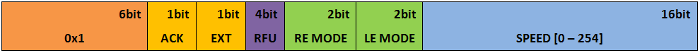
\includegraphics[width=\textwidth]{../images/appendix/cmd_0x01.png}
 \caption{Schemat ramki odpowiedzialnej za sterowanie silnikami}
 \label{fig:CMD_0x01}
\end{figure}

\subsection{Sterowanie serwomechanizmem}
\begin{figure}[h!] 
 \centering
 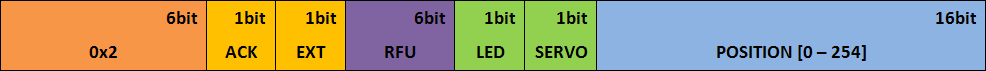
\includegraphics[width=\textwidth]{../images/appendix/cmd_0x02.png}
 \caption{Schemat ramki odpowiedzialnej za sterowanie silnikami}
 \label{fig:CMD_0x02}
\end{figure}

Szczegóły:
\begin{description}[itemsep=0pt,topsep=0pt, partopsep=0pt]
\item[Biology] Study of life
\item[Physics] Science of matter and its motion.
\item[Psychology] Scientific study of mental processes and behaviour.
\end{description}

\section{Komunikaty specjalne}